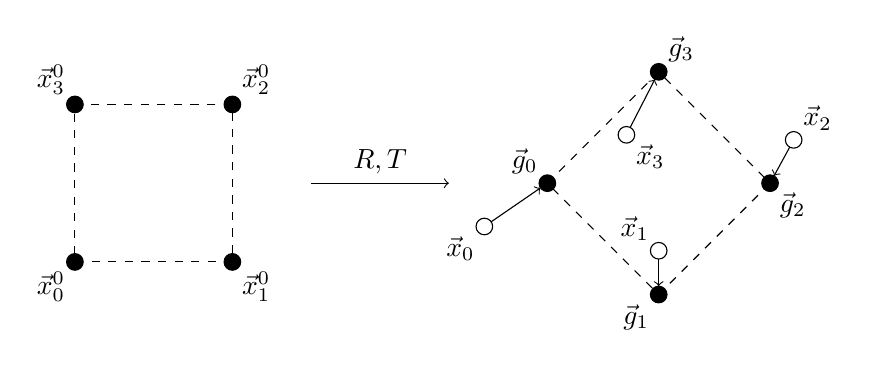
\begin{tikzpicture}

	\coordinate (A) at (0, 0, 0);
	\coordinate (B) at (2, 0, 0);
	\coordinate (C) at (2, 2, 0);
	\coordinate (D) at (0, 2, 0);

	\draw[-,dashed] (A) -- (B) -- (C) -- (D) -- (A);

	\filldraw[fill=black, draw=black] (A) circle (3pt);
	\filldraw[fill=black, draw=black] (B) circle (3pt);
	\filldraw[fill=black, draw=black] (C) circle (3pt);
	\filldraw[fill=black, draw=black] (D) circle (3pt);

	\node[above left] at (D) {$\vec{x}^0_3$};
	\node[below right] at (B) {$\vec{x}^0_1$};
	\node[above right] at (C) {$\vec{x}^0_2$};
	\node[below left] at (A) {$\vec{x}^0_0$};

	% arrow
	\coordinate (R1) at (3, 1, 0);
	\coordinate (R2) at (4.75, 1, 0);
    \draw[->] (R1) -- (R2) node[midway,above] {$R, T$};

	% transformed

	\coordinate (A1) at (6, 1, 0);
	\coordinate (B1) at (7.4142, 2.4142, 0);
	\coordinate (C1) at (8.8284, 1, 0);
	\coordinate (D1) at (7.4142, -0.4142, 0);

	\draw[-,dashed] (A1) -- (B1) -- (C1) -- (D1) -- (A1);

	\filldraw[fill=black, draw=black] (A1) circle (3pt);
	\filldraw[fill=black, draw=black] (B1) circle (3pt);
	\filldraw[fill=black, draw=black] (C1) circle (3pt);
	\filldraw[fill=black, draw=black] (D1) circle (3pt);

	\node[below left] at (D1) {$\vec{g}_1$};
	\node[above right] at (B1) {$\vec{g}_3$};
	\node[below right] at (C1) {$\vec{g}_2$};
	\node[above left] at (A1) {$\vec{g}_0$};

	\coordinate (X1) at (5.2, 0.45, 0);
	\coordinate (X2) at (7.0042, 1.6142, 0);
	\coordinate (X3) at (9.1284, 1.55, 0);
	\coordinate (X4) at (7.4142, 0.142, 0);

	\filldraw[fill=white, draw=black] (X1) circle (3pt);
	\filldraw[fill=white, draw=black] (X2) circle (3pt);
	\filldraw[fill=white, draw=black] (X3) circle (3pt);
	\filldraw[fill=white, draw=black] (X4) circle (3pt);

	\node[below left] at (X1) {$\vec{x}_0$};
	\node[below right] at (X2) {$\vec{x}_3$};
	\node[above right] at (X3) {$\vec{x}_2$};
	\node[above left] at (X4) {$\vec{x}_1$};

    \draw[shorten >=3pt,shorten <=3pt,->] (X1) -- (A1);
    \draw[shorten >=3pt,shorten <=3pt,->] (X2) -- (B1);
    \draw[shorten >=3pt,shorten <=3pt,->] (X3) -- (C1);
    \draw[shorten >=3pt,shorten <=3pt,->] (X4) -- (D1);

\end{tikzpicture}
